\chapter{Online ranking algorithms}
\label{ch:online_ranking}
\textbf{Online ranking algorithms} do not rely on obtaining information about all previous matches, they only need the last state of players' ratings to be able to update them. Therefore, they update players' ratings after every match that is played, not in a batch after some period.
 
The advantage of online ranking algorithms is that it is not required to process all matches when updating ratings, which can become computationally difficult for bigger datasets.

On the contrary, since all of the previous outcomes have to be captured by one state, it may become difficult to precisely capture all previous matches and some information may be lost.

\section{Elo for 2 players}
\label{ch:elo_for_two_players}
Elo is a ranking system used for 2-player games, originally in chess. It was introduced in 1959 by an amateur chess player Arpad Elo \citep{Eloratingchessplayerspresent1978}. It has been used in chess ever since, and because of its success and simplicity, people have started using Elo also for different sports.

The Elo ranking algorithm assumes that player's skill is normally distributed, with the mean of the distribution representing player's most probable skill. Although the original Elo system assumes a homogeneous normal distribution among all players, it was later observed that logistic distribution fits the chess data better \citep{ReganUnderstandingDistributionsChess2011} as well as it is computationally less complex. Therefore, the logistic distribution has been used for chess ratings.

\subsection{Expected score}
\label{sec:expected_score}
Elo's expected score equation is based on logistic function. It is used to calculate player's expected performance given both his and his opponent's ratings. The player's expected performance can also be viewed as his probability of defeating his opponent and it can be calculated as follows.

\begin{equation}
E_A = \frac{1}{1+10^\frac{R_B-R_A}{400}},
\label{eq:expected_score}
\end{equation}

\noindent with players $A$ and $B$ of ratings $R_A$ and $R_B$, respectively, expected score $E_A$ of player $A$ can be calculated.

As mentioned, the formula was originally based on logistic distribution, which assumes lesser chance of more extreme players winning/losing as shown in \autoref{fig:log_vs_normal}.

\begin{figure}[H]
\centering
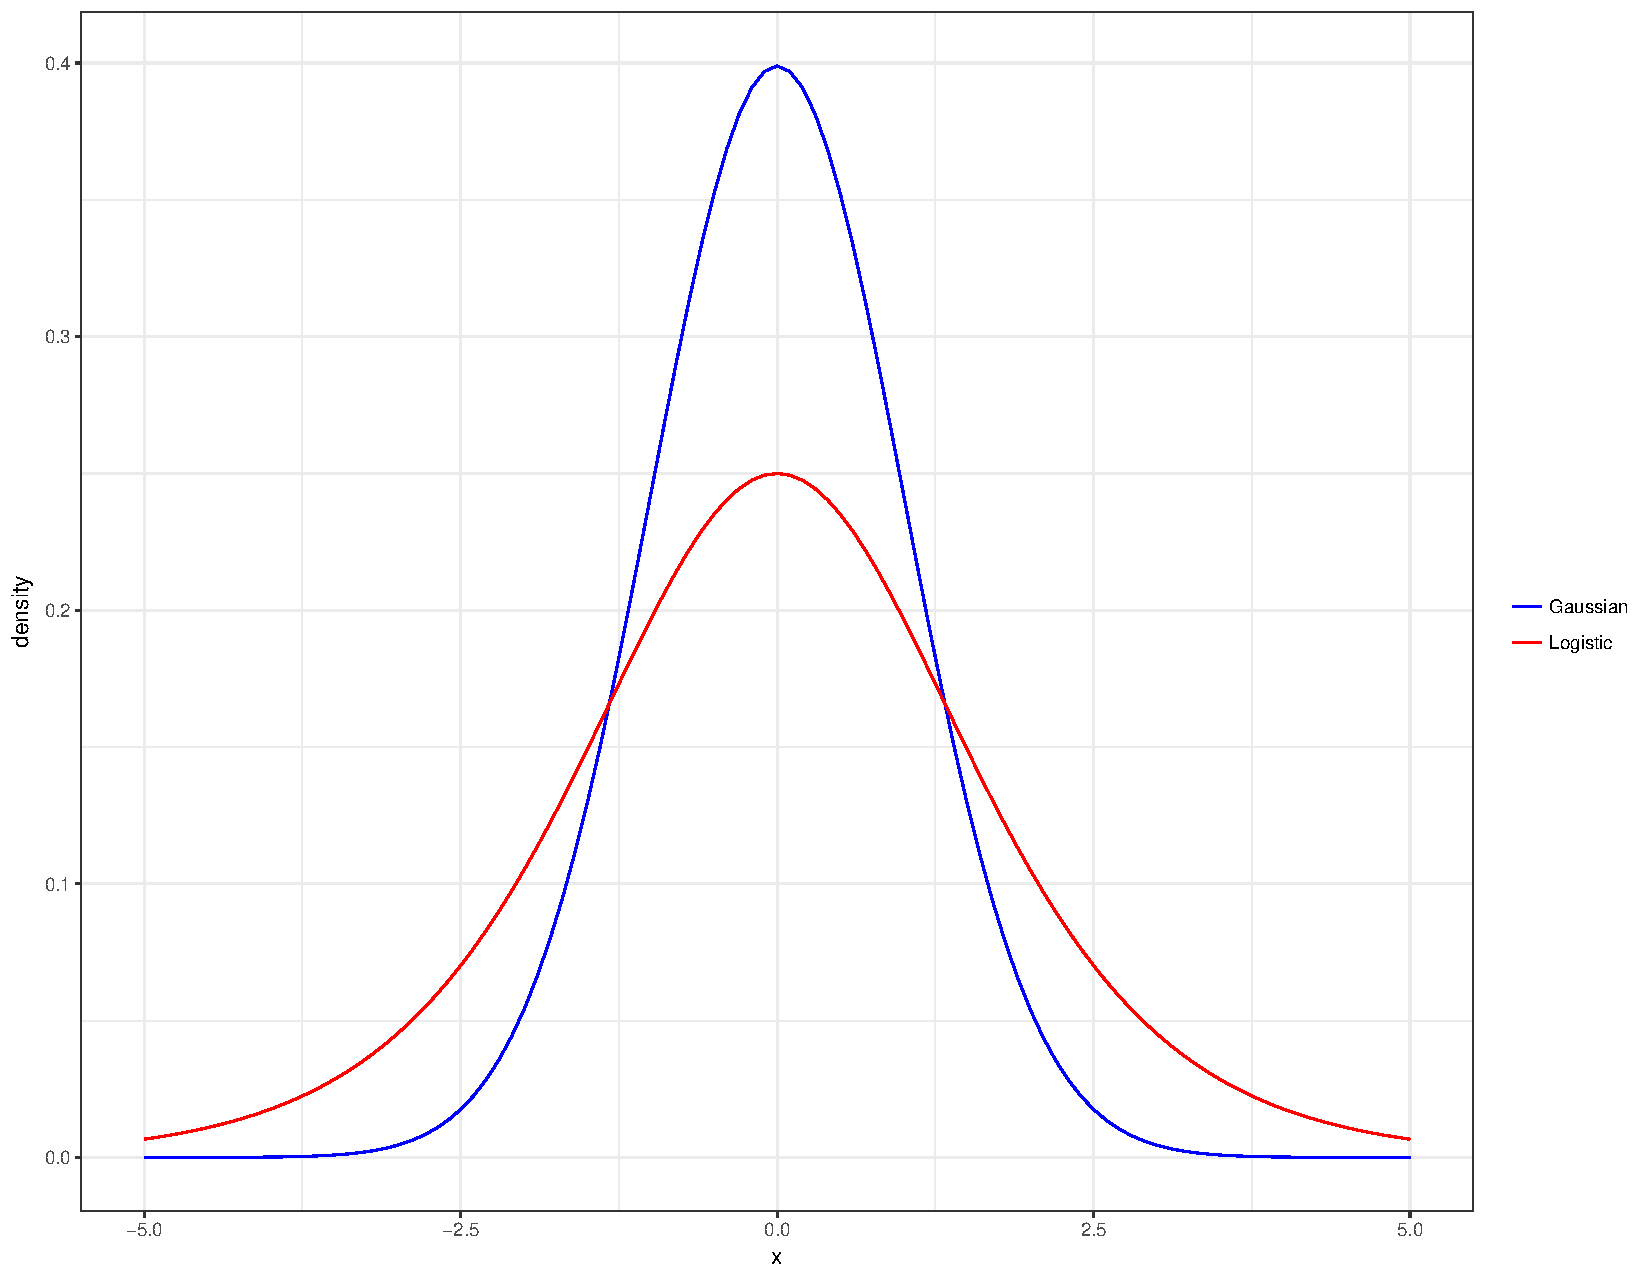
\includegraphics[width=0.8\textwidth]{figs/logistic_vs_gauss}
\caption{Difference between logistic and normal distribution}
\label{fig:log_vs_normal}
\end{figure}

The difference of 200 Elo points makes for a winning chance of \textasciitilde 76\% and is thought of as of a \textit{skill group}. The constants in the equation make the logistic function meet this rule as well as fit the actual chess players' data.

\begin{figure}[H]
\centering
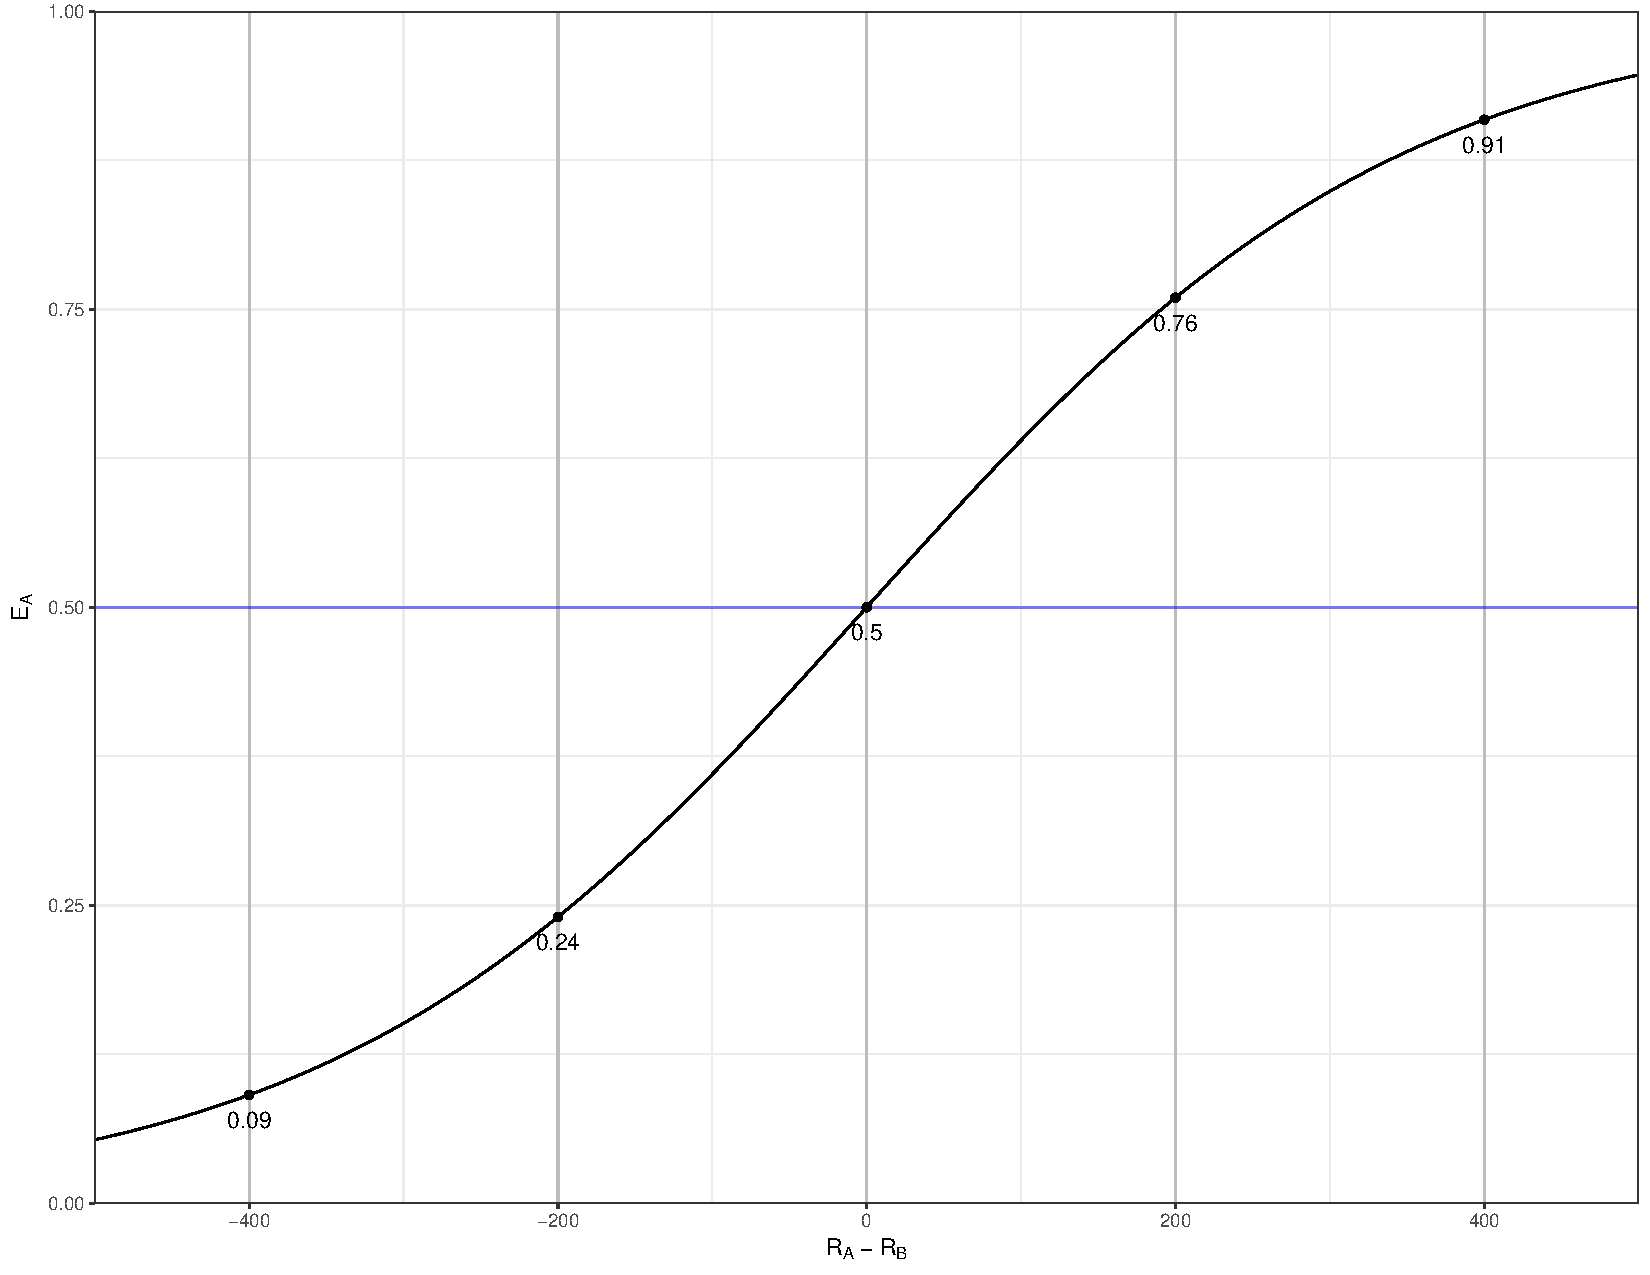
\includegraphics[width=0.8\textwidth]{figs/elo_logistic_function}
\label{Expected score equation}
\caption{Probability of winning based on rating difference}
\end{figure}

Since player's skill is thought of as a random variable, the logistic function can be perceived as the distribution of such random variable and therefore, a match of two players makes for a random variable of match's outcome and can be obtained by taking the difference of players' ratings.

Because $E_A$ and $E_B$ can be thought of as of probabilities of players $A$ and $B$ winning the game, it is intuitively a desired behavior that $E_A + E_B = 1$. The expected score formula, of course, meets this requirement.

Let $R_A$ and $R_B$ represent the rating of the players $A$ and $B$, respectively, then $E_A + E_B = 1$.

\begin{proof}
\begin{equation*}
\begin{aligned}
\frac{1}{1+10^{\frac{R_B-R_A}{400}}} + \frac{1}{1+10^{\frac{R_A-R_B}{400}}} &= 1\\[1em]
1+10^\frac{R_B-R_A}{400} + 1+10^\frac{R_A-R_B}{400} &= \left(1+10^\frac{R_B-R_A}{400}\right)\cdot\left(1+10^\frac{R_A-R_B}{400}\right)\\ [1em]
10^{\frac{R_B-R_A}{400}} \cdot 10^{\frac{R_A-R_B}{400}} &= 1\\[1em]
10^{\frac{R_B-R_A}{400} + \frac{R_A-R_B}{400}} &= 1\\[1em]
10^0 &= 1\\[1em]
1 &= 1
\end{aligned}
\end{equation*}
\end{proof}

Moreover, a little adjustment of the equation \eqref{eq:expected_score} reveals that Elo is a~derivation of the Bradley-Terry mode l\eqref{eq:bradley_terry}.

\begin{equation*}
\begin{aligned}
E_A &= \frac{1}{1 + 10^{\frac{R_B-R_A}{400}}} \\[1em]
&= \frac{1}{1 + 10^{\frac{R_B}{400}-\frac{R_A}{400}}} \\[1em]
&= \frac{1}{1 + \frac{10^{\frac{R_B}{400}}}{10^{\frac{R_A}{400}}}}\cdot \frac{10^{\frac{R_A}{400}}}{10^{\frac{R_A}{400}}} \\[1em]
&= \frac{10^{\frac{R_A}{400}}}{10^{\frac{R_A}{400}}+10^{\frac{R_B}{400}}} \\[1em]
&= \frac{p_A}{p_A + p_B}
\end{aligned}
\end{equation*}

Therefore, Elo is based on the Bradley-Terry model, with variables $p_A$ and $p_B$ representing scores of players $A$ and $B$, respectively. Therefore, in Elo, score of player $A$ is obtained as $10^\frac{R_A}{400}$, where $R_A$ holds his current rating.

\subsection{Updating ratings}
After the outcome of the game is known, players' ratings are updated accordingly. Intuitively, if a weak player beats a strong player, the weak player's rating should increase a lot, while the strong player's should decrease a lot. Similarly, if a strong player defeats a weak player, the weaker player should not be punished that much. In other words, results that are expected by the system should not lead to big changes in players' ratings, while unexpected results should.

In the Elo, following equation is used to update player's rating

\begin{equation}
R_A' = R_A + K(S_A - E_A),
\label{eq:update_equation}
\end{equation}

\noindent where $R_A$ is player's rating before the update, $E_A$ is player's expected score calculated from expected score formula \eqref{eq:expected_score} and $S_A$ is player's actual score, which can hold 3 different values:

\begin{itemize}
\item $1$ if player A won, 
\item $0$ if he lost,
\item $0.5$ if the game ended in a draw.
\end{itemize}

Finally, the $K$ is called $K$ factor and represents the maximum value a player can either lose or gain. The $K$ factor can vary depending on player's rating as described in \eqref{sec:k_factor}.

The equation \eqref{eq:update_equation} fits the requirements for an update formula as more unexpected results lead to more extreme changes while predictable results update the ratings by lower values.

In \autoref{fig:k_factor}, the change in player's rating based on difference of both players' ratings using $K$ factor of 32 is indicated.

\begin{figure}[H]
\centering
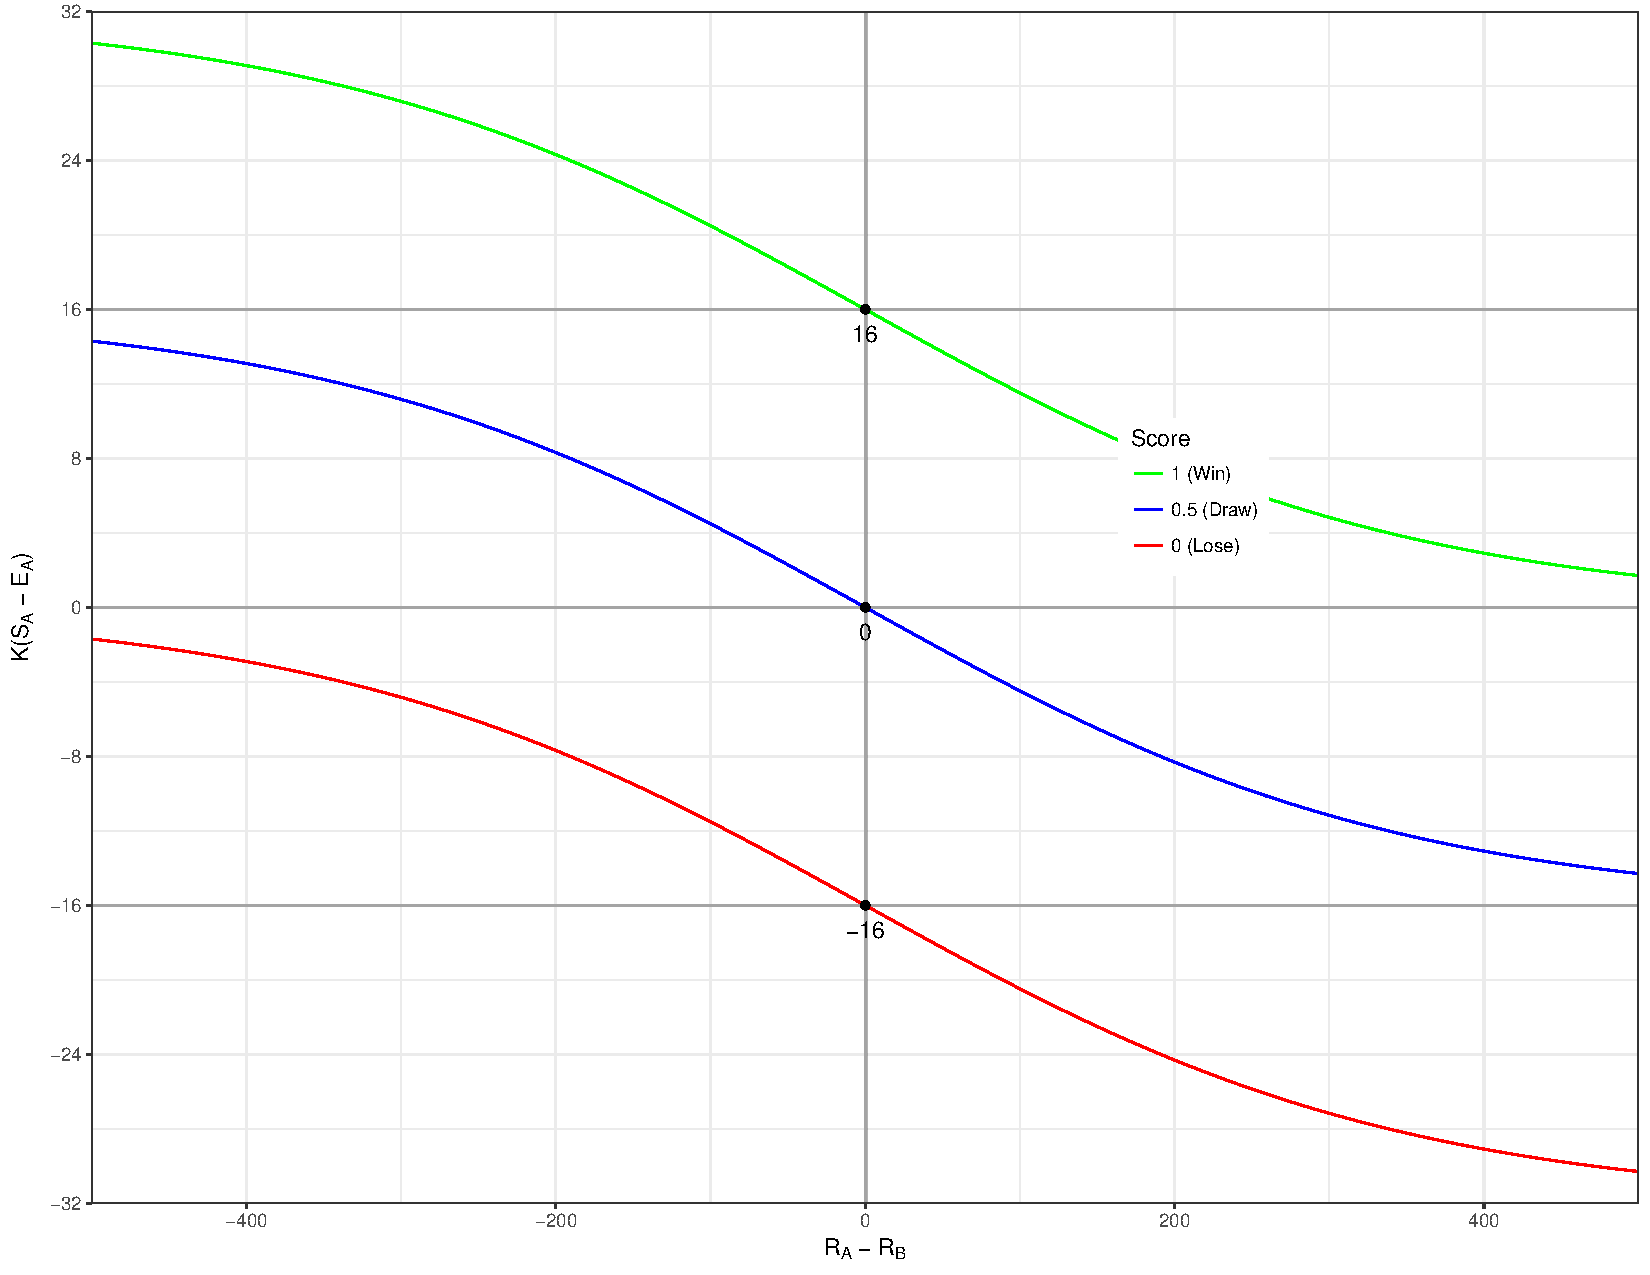
\includegraphics[width=0.8\textwidth]{figs/elo_k_factor}
\caption{Change in rating for K factor of 32}
\label{fig:k_factor}
\end{figure}

\subsection{K factor}
\label{sec:k_factor}
As the $K$ factor defines the maximum possible update of a player's rating after one game, having such parameter fixed leads to the lack of ability to recognize player's true skill in shorter time and dynamically respond to that. To provide an example, player's increased number of victories likely points to player's higher true skill, since he tends to defeat players with ratings similar to his. The system should be able to react to such situations by increasing the player's rating by higher values until he eventually reaches his true skill and stabilizes.

The USCF and FIDE solve this by dividing players into three categories based on their rating and setting a different value of $K$ factor for every category. That makes it easier for new players to achieve rating according to their actual skill and once their rating reaches a pre-set value, they get artificially settled by setting their $K$ factor to a lower value. Note that FIDE sets $K$ factor to 10 after a player reaches rating of 2400 and then the player is considered settled, therefore his $K$ factor stays at 10 even if the player manages to reduce his rating back under 2400.

\examplespace
\begin{example}
For an example of the Elo rating system, let's have a match of two imaginary players Alice and Bob with ratings 1170 and 1290, respectively. The probability of Alice defeating Bob $E_A$ will be calculated as follows.

\begin{align*}
E_A &= \frac{1}{1+10^{\frac{R_B-R_A}{400}}} \\
&= \frac{1}{1+10^{\frac{1290-1170}{400}}} \\ 
&= \frac{1}{1+10^{\frac{120}{400}}} \\[0.5em]
&\doteq 0.334
\end{align*}

Therefore, Alice's chances of beating Bob are around 33.4\%. Complementarily, Bob's chances are about 66.6\%. Let's say Alice beats her odds and defeats Bob. Assuming $K$ factor of 32, her rating will be update as follows. 

\begin{align*}
R_A' &= R_A + K(S_A - E_A) \\
&= 1170 + 32(1 - 0.334) \\
&\doteq 1191.3
\end{align*}

In the same spirit, Bob's rating will decrease as follows.

\begin{align*}
R_A' &= R_A + K(S_A - E_A) \\
&= 1290 + 32(0 - 0.666) \\
&\doteq 1268.7
\end{align*}

If they were to play the same match again with updated ratings, the system would expect Alice to defeat Bob with a \textasciitilde 39\% chance.
\end{example}

\section{Extensions to the Elo algorithm}
\label{section:elo_for_teams}
In this chapter we provide a heuristic algorithm to derive an extension of the Elo ranking algorithm for teams with multiple players. This consists of computing individual player Elo scores and aggregating them to produce an Elo score for the team. Winning likelihoods are then computed.

\subsection{Altering the classification rule by number of draws}
As the Bradley-Terry model is used for calculating expected score in the Elo ranking system, only probabilities of winning or losing can be obtained. However, in sports, it is often desired for draws to be considered. As \citet{RaoTiesPairedComparisonExperiments1967} suggested, the Bradley-Terry model can be extended to account for ties by introducing $\theta \geq 1$ parameter. Then, the Rao-Kupper model captures the preference of $i$-th player over $j$-th player and vice versa in dependence on their skills $\pi_i$, $\pi_j$, respectively, as

\begin{align*}
P(i > j) &= \frac{\pi_i}{\pi_i + \theta\pi_j},\\
P(j > i) &= \frac{\pi_j}{\pi_j + \theta\pi_i}
\end{align*}

\noindent and the probability of a game between $i$-th and $j$-th player resulting in a tie can be expressed as

\begin{align*}
P(i = j) = \frac{(\theta^2 - 1)\pi_i\pi_j}{(\pi_i+\theta\pi_j)(\pi_j+\theta\pi_i)}.
\end{align*}

The $\theta$ parameter is chosen accordingly to the frequency of ties in given sport. While in soccer draw is a common outcome of a match and therefore the $\theta$ is desired to be high, for instance in Olympic swimming, swimmers are considered to draw if their times are tied to a hundredth of a second, making draws much less often. Hence, for swimming, the $\theta$ parameter should be smaller, making prediction of a draw less probable.

To obtain the $\theta$ parameter for the data used throughout this thesis, minimization of function $f(\theta)$ as shown in \eqref{eq:rao_kupper_minimization} has been performed.

\begin{align}
\label{eq:rao_kupper_minimization}
f(\theta) = \frac{1}{|M|}\nsum_{i \in M}{
\begin{bmatrix}
o_{i_w} & o_{i_\ell} & o_{i_d}
\end{bmatrix}
\times
\begin{bmatrix}
p_{i_w}\cdot\log{p_{i_w}} \\
p_{i_\ell}\cdot\log{p_{i_\ell}} \\
p_{i_d}\cdot\log{p_{i_d}}
\end{bmatrix}
},
\end{align}

where $i \in M$ denotes $i$-th match from the set of all matches $M$, $o_{i_w}$, $o_{i_\ell}$, $o_{i_d}$ its outcome in the sense that $o_{i_w} = 1, o_{i_\ell} = o_{i_d} = 0$ if the team won and correspondingly for loses and draws, and $p_{i_w}$, $p_{i_\ell}$, $p_{i_d}$ probabilities of winning, losing and drawing, respectively, predicted by the Rao-Kupper model.

By minimizing $f(\theta)$, a result of $\theta \doteq 1.326$ has been obtained. However, we believe that the draws in used dataset are not sufficiently significant and the obtained result does not reflect the reality, making the Rao-Kupper model unusable for the dataset. To support the statement, probability of a draw of two players $i$ and $j$ of equal ratings $R_i = R_j = 1200$ is calculated using $\theta = 1.326$:

\begin{align*}
P(i = j) &= \frac{\left(1.326^2 - 1\right)10^{1200/400}10^{1200/400}}{\left(10^{1200/400}+1.326\cdot 10^{1200/400}\right) \left( 10^{1200/400}+1.326\cdot 10^{1200/400}\right) } \\[1em]
&\doteq 0.14.
\end{align*}

While the probability of a draw is at its peak for a match of players of equal ratings, the probability has been calculated to 14\%. For players of different ratings, the probability will only get lower. However, draws make up for a total of \textasciitilde 23\% of all matches in the dataset, pointing to a conclusion that Rao-Kupper is not usable for our dataset.

\subsection{Parameter optimization for prediction}
Since the Elo algorithm was adjusted to fit the chess data, the expected score equation \eqref{eq:expected_score} uses two constants that we try to adjust accordingly to soccer data. In order to do that, we maximize the prediction ability of expected score equation using derivative-free methods.

\subsubsection{Simulated annealing}
\label{sec:simulated_annealing}
Simulated annealing is a probabilistic technique for finding the global optimum of a function introduced by \citet{KirkpatrickOptimizationSimulatedAnnealing1983}. The algorithm starts with an initial temperature and while searching the space, it slowly cools down. With lower temperature comes lower probability of getting stuck in a local optimum. Therefore, the algorithm tends to neglect local optima. When the algorithm cools down, making it unable to escape local optima, it stops.

More thorough explanation of the simulated annealing algorithm is provided in \autoref{ch:simulated_annealing}.

After determining players' ratings, simulated annealing algorithm is used to alter the expected score equation \eqref{eq:expected_score} to maximize number of correctly predicted matches. Therefore, $x$ and $y$ in formula \eqref{eq:expected_score_altered} are adjusted in order to maximize algorithm's prediction ability.

\begin{equation}
\label{eq:expected_score_altered}
E'_A = \frac{1}{1+x^\frac{R_B-R_A}{y}}.
\end{equation}

Another approach is to minimize the formula's log-likelihood loss function \citep{BujaLossFunctionsBinary2005} using simulated annealing. Although, log-likelihood loss function and number of correctly predicted matches tend to be correlated, and therefore both approaches lead to similar results.

\subsubsection{Cross-entropy method}
Cross-entropy method is a Monte Carlo approach to global optimization introduced by  \citet{RubinsteinCrossEntropyMethodCombinatorial1999}. In order to find the global optimum, a random data sample is generated according to a parameter, from which only the most elite percentage is chosen and the parameter to generate the data sample with is updated according to the elite. This process is repeated multiple times to obtain the global optimum.

Again, more detailed information on cross-entropy method can be read at \autoref{ch:cross_entropy_method}.

In the case of optimizing Elo's parameters, 100 random samples from a two dimensional normal distribution with the Elo's equation's constants $x$ and $y$ from \eqref{eq:expected_score_altered} is generated and the average of the most elite 20\% of such is used to update the parameters. This process is repeated 100 times.

To optimize Elo's parameters using cross-entropy method, the cross-entropy error function \citep{deBoerTutorialCrossEntropyMethod2005} of correctly predicted matches is used as the fitness function. The cross-entropy error function in general case looks as follows.

\begin{equation*}
H(p, q) = -\sum_i{p_i\log{q_i}}.
\end{equation*}

And therefore, for Elo's parameter optimization:

\begin{equation*}
H(w, p) = -\sum_i{(w_i\cdot\log{p_i} + (1-w_i)\cdot\log{(1-p_i)})},
\end{equation*}

\noindent where $w_i$ equals to 1 if the home team won the match, 0 otherwise, and $p_i$ is the probability of home team winning the game predicted by the Elo model.

Since both of those algorithms are used to find the global maximum of the Elo's equation, they both had similar results. Again, since there is a fair amount of randomness included, there is no point in saying whether one of them was slightly better.

\subsection{Using normal distribution}
Although the Elo rating system follows the logistic distribution for calculating expected score of a player, as mentioned in \ref{sec:expected_score}, the original formula proposed by Arpad Elo used a normal distribution. The reason it was disregarded in favor of logistic distribution was that the latter captured the chess data more accurately.

Because we use soccer data, it is reasonable to use the normal distribution $\mathcal{N}(\mu, (2000/7)^2)$ proposed by Arpad Elo. The distribution assumes that players' ratings are homogeneously distributed and uses a constant deviation $\sigma=\frac{2000}{7}$. The mean $\mu$ is equal to given player's rating.

\subsection{Treating teams as individuals}
An intuitive way to extend the Elo algorithm to be able to calculate team ratings is to treat every team as an individual. This approach leads to having team rating based purely on match outcomes with no respect to the team's players' individual skills. Therefore, with unstable team lineups, predicting future games turns out to be challenging. 

Although, to provide an intuitive comparison to the approach presented in \ref{sec:elo_team_ranking}, real data has been evaluated using this approach as well.

\subsection{Adaption for team ranking}
\label{sec:elo_team_ranking}
To extend Elo to be able to rank teams, teams are perceived as individual players. However, team ratings are determined from individual players' ratings and after the team's rating is updated, the update is propagated back to players' ratings. The propagation has to ensure consistency of ratings, i.e. the rule applied to calculate team's rating from players' ratings has to be applicable and equivalent to the team's updated rating after the update.

\subsubsection{Obtaining team's rating}
The goal of obtaining team's rating is to obtain such rating that captures the team's skill (i.e. its players' joined skills) as accurately as possible. It may seem useful to introduce new attributes of the obtained rating, for example deviation of players' ratings, but it is essential to use the rest of the Elo formulas without further complicated alterations.

Therefore, we obtain team's rating by calculating arithmetic mean of all players' ratings that belong to the team. This lets the team's rating remain on the same scale as players' ratings and therefore be suitable for other Elo equations without further adaptations. Also, every player's rating affects the team's rating equally. A downside of such approach is the difficulty of comparing quantitatively unbalanced teams. Although, quantitatively unbalanced soccer matches are rare and therefore we believe that formula \eqref{eq:obtaining_teams_rating} is suitable for calculating team's rating.

\begin{equation}
\label{eq:obtaining_teams_rating}
R_{T_i} = \frac{1}{|T_i|}\sum_{R_j \in T_i}{R_j},
\end{equation}

\noindent where $T_i$ is a set of all ratings of all players in $i$-th team and $|T_i|$ is size of such set (i.e. number of players in the team).

\subsubsection{Applying Elo's equations}
The obtained teams' ratings can be treated as ratings of individuals and therefore expected score equation \eqref{eq:expected_score} and update equation \eqref{eq:update_equation} can be applied on them.

Treating teams as individuals and applying the same equations to them as in Elo for two players, and keeping the consistency between team ratings and player ratings, leads to similar behavior as in Elo for two players and therefore makes it a suitable expansion.

For completeness, below is the update formula.

\begin{equation}
\label{eq:teams_update}
R_{T_i}' = R_{T_i} + K(S_{T_i} - E_{T_i}),
\end{equation}

\noindent with $R_{T_i}'$ and $R_{T_i}$ being the new and old rating of $i$-th team, respectively, $S_{T_i}$ its actual score, $E_{T_i}$ expected score and $K$ the K-factor.

\subsubsection{Propagating updated rating to players}
To satisfy the consistency between teams' ratings and players' ratings, players' ratings could be updated by the same rating as the team's rating is. Although, because matches tend to be played between teams of similar level, weaker players play a game of higher rating than their own and in consequence the game is harder for them. This is accordingly taken into account and weaker players are punished less if the team loses and rewarded more if the team wins. Moreover, to satisfy the consistency of ratings, opposite rule is applied to stronger players. Also, this leads to converging players' ratings to the team rating, which is also a desired behavior, since team's rating better captures its actual skill if its players are of similar skill. \linebreak To satisfy such behavior, we propose following formula to propagate updated rating $R'_{T_i}$ of $i$-th team to its $j$-th player.

\noindent
\begin{proposition}
Let $R_j$ and $R'_j$ represent $j$-th player's rating before and after update, respectively, and $R_{T_i}$ and $R_{T_i}'$ $i$-th team's rating obtained from \eqref{eq:obtaining_teams_rating} and \eqref{eq:teams_update}. Also, let $S_{T_i}$ represent the outcome of the game, relatively to the $j$-th team,

\begin{itemize}
\item 1 if $j$-th team won the game,
\item 0 if $j$-th team lost the game,
\item 0.5 if the game was tied.
\end{itemize}

\noindent It follows that $R'_j$ is obtained as

\begin{equation}
\label{eq:propagating_rating_to_players}
R_j' = R_j + (R_{T_i}' - R_{T_i})\left(\frac{R'_{T_i} - (2S_{T_i}-1)(R_j-R_{T_i})}{R'_{T_i}}\right).
\end{equation}

\noindent This formula satisfies the consistency requirement.
\end{proposition}

\begin{proof}
Since
\begin{align}
R'_{T_i} &= R_{T_i} + K(S_{T_i} - E_{T_i}), \label{eq:eft_update_team}\\[1em]
R_{T_i} &= \frac{1}{|T_i|}\sum_{R_j \in R_{T_i}} R_j, \label{eq:eft_team_rating}\\
R'_j &= R_j + (R_{T_i}' - R_{T_i})\left(\frac{R'_{T_i} - (2S_{T_i}-1)(R_j-R_{T_i})}{R'_{T_i}}\right),
\end{align}
to prove that the consistency requirement holds true, we need to show that
\begin{align*}
R'_{T_i} = \frac{1}{|T_i|} \nsum_{R_j \in R_{T_i}}{R_j + (R_{T_i}' - R_{T_i})\left(\frac{R'_{T_i} - (2S_{T_i}-1)(R_j-R_{T_i})}{R'_{T_i}}\right)}.
\end{align*}
Hence from \eqref{eq:eft_update_team}, \eqref{eq:eft_team_rating}
\begin{align*}
K(S_{T_i} - E_{T_i}) &= \frac{K(S_{T_i} - E_{T_i})}{|T_i|}\nsum_{R_j \in R_{T_i}}{\frac{R'_{T_i} - (2S_{T_i}-1)(R_j-R_{T_i})}{R'_{T_i}}} \\[1em]
1 &= \frac{1}{|T_i|}\nsum_{R_j \in R_{T_i}}{\frac{R'_{T_i} - (2S_{T_i}-1)(R_j-R_{T_i})}{R_{T_i}}} \\[1em]
1 &= \frac{1}{|T_i|}\left(\nsum_{R_j \in R_{T_i}}\frac{R'_{T_i}}{R_{T_i}} - (2S_{T_i}-1)\nsum_{R_j \in R_{T_i}}\frac{R_j-R_{T_i}}{R'_{T_i}}\right) \\[1em]
1 &= 1-\frac{1}{|T_i|}(2S_{T_i}-1)\left(\nsum_{R_j \in R_{T_i}}\frac{R_j}{R'_{T_i}}-\nsum_{R_j \in R_{T_i}}\frac{R_{T_i}}{R'_{T_i}}\right) \\[1em]
0 &= \nsum_{R_j \in R_{T_i}}\frac{R_j}{R'_{T_i}}-\nsum_{R_j \in R_{T_i}}\frac{R_{T_i}}{R'_{T_i}} \\[1em]
0 &= \frac{1}{R'_{T_i}}|T|R_{T_i} - \frac{R_{T_i}}{R'_{T_i}}|T| \\[1em]
0 &= 0,
\end{align*}
which ultimately holds true and therefore, the formula \eqref{eq:propagating_rating_to_players} satisfies the consistency requirement.
\end{proof}

\subsection{Applying Elo for teams on real data}
To determine the quality of the Elo extension for teams, the algorithm was applied on real soccer data. Every player was assigned an initial rating of 1200 and throughout the matches, with ratings of players still being determined, Elo's expected score formula \eqref{eq:expected_score} was applied to predict the outcomes of the matches.

It is important to keep in mind what a random game soccer is and therefore how unforeseeable soccer matches are. Although the bookmakers managed to predict 53\% outcomes correctly \citep{EuropeanSoccerDatabase}, the Elo for teams adaptation predicted correctly about 41.93\% matches.

However, since the classification is not binary, both number of correctly predicted matches and \textbf{log-likelihood loss function} is used for result comparison. To compute the log-likelihood loss, following formula is used.

\begin{equation*}
\label{eq:log_likelihood}
-\frac{1}{n} \sum_{i=1}^{n} w_i\cdot \log{e_i} + (1-w_i)\cdot \log{(1-e_i)},
\end{equation*}

\noindent where $w_i$ equals to 1 if home team won the match and 0 otherwise, $e_i$ is the expected score predicted by Elo model \eqref{eq:expected_score} and $n$ is the number of matches. Since with increasing error on prediction the log-likelihood increases as well, the goal is to minimize log-likelihood loss.

The log-likelihood does not provide much information without comparison to other results, hence it is stated in \autoref{table:elo_results} alongside with other results.

\subsection{Using prior knowledge}
The dataset contains knowledge that could be used to improve Elo's ability to predict the correct outcome of a match. In the following sections, the knowledge will be described as well as its application to Elo. A more detailed description of the dataset knowledge used in this section is described in \ref{sec:data_analysis}.

\subsubsection{Overall rating}
\label{sec:overall_rating}
Skill of players in the dataset is estimated by the overall rating attribute, which expresses how well has given player performed. Such value can be used to initialize players' ratings to help Elo find players' true skill faster. Since the attribute is represented as a value from the interval $[0, 100]$, a normalization onto an interval appropriate to the Elo scale is necessary.

Since the default rating used for Elo system is 1200 and difference of 200 rating makes for a \textasciitilde 76\% chance of winning, after several tests, the interval to normalize overall rating onto has been chosen as $[1000, 1400]$ as a compromise that is both conservative and effective.

\subsubsection{Initializating with statistics using Bayes' formula}
Despite the home-team advantage phenomena, Elo's prediction formula gives both teams equivalent chances of winning. Since around 45.9\% matches in used dataset are won by the home team, while around 28.8\% by the away team, such information can be used to alter the home team's expectation score in following way.

\begin{align*}
P(A\ wins \mid A\ is\ home) &= \frac{P(A\ is\ home \mid A\ wins)\cdot P(A\ wins)}{P(A\ is\ home)}\\
P(A\ is\ home \mid A\ wins) &= 0.614\\
P(A\ wins) &= e_A\\
P(A\ is\ home) &= 0.5\\
P(A\ wins \mid A\ is\ home) &= \frac{0.614\cdot e_A}{0.5} = 1.228\cdot e_A\\
\end{align*}

\noindent where $e_A$ is the probability of team A winning calculated by the Elo equation. $P(A\ is\ home \mid A\ wins)$ is calculated as the ratio of number of matches when A was home and number of all matches that ended as either a victory or a loss. Note that draws are disregarded.

\subsection{Predicting outcome after ratings have been determined}
Since the quality of the algorithm is judged by its ability to predict outcomes of matches, it is troubling that every player is assigned the same initial rating. The number of games an average player has played in used dataset is 25, which clearly leads to inaccuracies, since according to \citet{Eloratingchessplayerspresent1978}, a player needs to have played at least 30 games before his rating reflects his skill. This makes a lot of matches be predicted at random and therefore impairs results of the experiments.

One way to overcome this issue was introduced in \ref{sec:overall_rating}, and although it improves the final prediction ability, assigning players ratings determined other way than by Elo defeats the purpose of measuring quality of Elo rating system.

A more accurate way is to calculate the number of correctly predicted games after players' ratings have been established. Although the ratings are correlated with games' outcomes and therefore it may not seem appropriate to judge the algorithm's quality this way, the amount of matches and soccer's randomness strongly helps to decorrelate the judged attributes.

To justify the statement, players have been trained on the dataset one hundred times and Elo's ability to predict outcomes was noted every iteration as shown in following figure.

\begin{figure}[H]
\centering
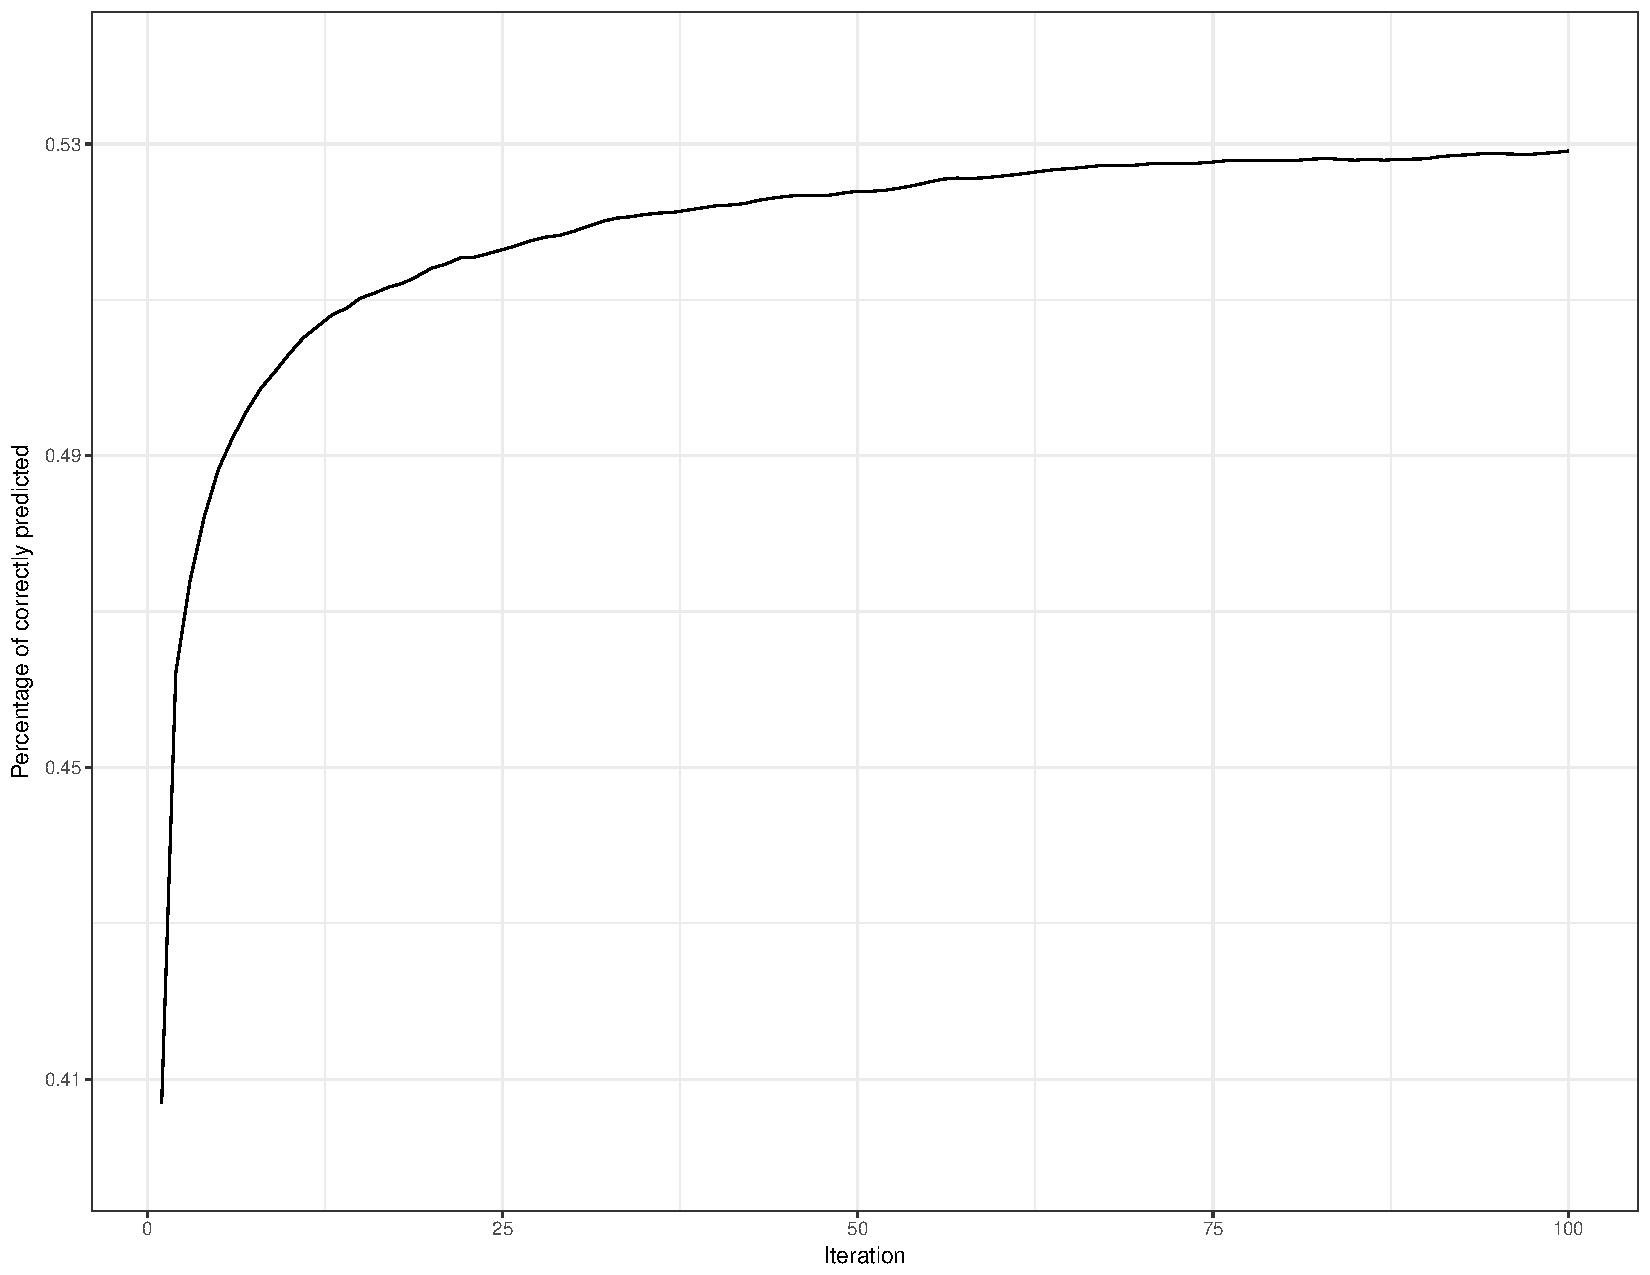
\includegraphics[width=0.8\textwidth]{figs/multiple_trainings}
\caption{Progress of prediction ability over multiple iterations}
\end{figure}

As shown in the graph, after the first iteration, the amount of randomly guessed outcomes has considerably lowered, which led to much better prediction ability. In the rest of the iterations, only slight improvements have been made, perhaps because of players with low number of matches played.

\subsection{Results}
In order to compare the quality of above-mentioned approaches, real soccer data have been evaluated with the intention of measuring the algorithms' ability to correctly predict future matches. Also, the log-likelihood loss is calculated as a different method of measurement. All approaches have been evaluated using both the logistic distribution used by chess players and normal distribution originally suggested by Arpad Elo.

Note that all values of prediction ability (PA) in \autoref{table:elo_results} are in percentage to provide a better picture about the ability.

Also, to provide a better perspective, it is worth noting that the state-of-the-art result of the prediction ability is around 53\% achieved by the bookkeepers. Results better than the state-of-the-art result are bold.

\begin{table}[H]
\caption{Prediction ability and log-likelihood loss of different approaches to Elo extensions}
\label{table:elo_results}
\centering
\begin{tabularx}{\textwidth}{ | l | X | X | X | X |}
\hline
& \multicolumn{2}{| c |}{\textbf{Logistic}} & \multicolumn{2}{| c |}{\textbf{Normal}} \\ \hline
& \textbf{PA} & \textbf{LL} &\textbf{PA} & \textbf{LL} \\ \hline
Treating teams as individuals & 44.59 & 0.638  & 44.23 & 0.634 \\ \hline
Pure extension & 46.22 & 0.615 & 44.03 & 0.621 \\ \hline
Parameter optimization & 46.54 & 0.615 & 44.21 & 0.620 \\ \hline
Overall rating & 46.50 & 0.613 & 44.41 & 0.619 \\ \hline
Ignoring draws & 51.64 & 0.615 & 51.58 & 0.621 \\ \hline
Bayes & \textbf{53.68} & 0.686 & 21.23 & 1.016 \\ \hline
PO \& OR \& Bayes & \textbf{53.72} & 0.691 & 21.02 & 1.042 \\ \hline
\end{tabularx}
\end{table}

\examplespace
\begin{example}
To provide an example of the extension for Elo, consider following lineups:

\begin{table}[H]
\centering
\begin{tabular}{l c c}
\textbf{Team} & \textbf{Player} & \textbf{Rating} \\
Team 1 ($T_1$) & Player A ($A$) & 1300 \\
& Player B ($B$) & 1400 \\
Team 2 ($T_2$) & Player C ($C$) & 1100 \\
& Player D ($D$) & 1000 \\
\end{tabular}
\end{table}

First of all, both $T_1$ and $T_2$ need to have the team rating calculated using \eqref{eq:obtaining_teams_rating}.

\begin{align*}
R_{T_1} &= \frac{1}{|T_1|}\sum_{R_j \in T_1}{R_j} \\
&= \frac{1}{2}(1300 + 1400) \\
&= 1350 \\[1.5em]
R_{T_2} &= \frac{1}{|T_2|}\sum_{R_j \in T_2}{R_j} \\
&= \frac{1}{2}(1100 + 1000) \\ 
&= 1050,
\end{align*}

\noindent obtaining ratings $R_{T_1} = 1350$ and $R_{T_2} = 1050$.

From here, the teams can be treated as individuals and therefore application of the expected score formula \eqref{eq:expected_score} produces expectancy of either team beating the other.

\begin{align*}
E_{T_1} &= \frac{1}{1+10^{\frac{R_{T_2} - R_{T_1}}{400}}} \\
&= \frac{1}{1+10^{-\frac{300}{400}}} \\
&\doteq 0.849 \\[1.5em]
E_{T_2} &= \frac{1}{1+10^{\frac{R_{T_1} - R_{T_2}}{400}}} \\
&= \frac{1}{1+10^{\frac{300}{400}}} \\
&\doteq 0.151,
\end{align*}

\noindent predicting that team $T_1$ will beat team $T_2$ with the probability of 0.849. This also makes intuitive sense if players' ratings of both teams are considered.
Say that team $T_2$ beat its odds and won the game. Considering $K$ factor of 32, this will affect the team ratings as follows.

\begin{align*}
R'_{T_1} &= R_{T_1} + K(S_{T_1} - E_{T_1}) \\
&= 1350 + 32(0 - 0.849) \\
&\doteq 1322.8 \\[1.5em]
R'_{T_2} &= R_{T_2} + K(S_{T_2} - E_{T_2}) \\
&= 1050 + 32(1 - 0.151) \\
&\doteq 1077.2,
\end{align*}

\noindent obtaining updated ratings $R'_{T_1} = 1322.8$ and $R'_{T_2} = 1077.2$.
Such ratings will then be propagated to the players $A$, $B$, $C$ and $D$. Propagation of the team rating to player $A$ is shown below while the procedure can be applied on other players analogously.

\begin{align*}
R'_A &= R_A + (R'_{T_1} - R_{T_1})\left(\frac{R'_{T_1} - (2S_{T_1} - 1)(R_A - R_{T_1})}{R'_{T_1}}\right) \\
&= 1300 + (1322.8 - 1350)\left(\frac{1322.8 - (0 - 1)(1300 - 1350)}{1322.8}\right) \\
&\doteq 1300 - 26.2 \\
& = 1273.8
\end{align*}

After applying the same procedure on other players, following table showing updated ratings of players and teams was produced.

\begin{table}[H]
\centering
\begin{tabular}{l c c c}
\textbf{Team} & \textbf{Team rating} & \textbf{Player} & \textbf{Player rating} \\
Team 1 ($T_1$) & 1322.83 & Player A ($A$) & 1273.86 \\
& & Player B ($B$) & 1371.80 \\
Team 2 ($T_2$) & 1077.17 & Player C ($C$) & 1125.91 \\
& & Player D ($D$) & 1028.54
\end{tabular}
\end{table}
\end{example}